\section{GitHub Copilot and AI Driven Development}
Introduced in 2021, GitHub's Copilot\footnote{https://copilot.github.com} is an in-IDE recommender system that leverages OpenAI's Codex~\cite{copilot} large language model (LLM) to generate code suggestions that are uncannily effective~\cite{copilot}. Codex and a similar product from Google, AlphaCode~\cite{alphacode}, are able to perform above human averages on programming contest problems, for example. It does not seem unreasonable to say that this will profoundly change the way we program.

What is less clear, at least for now, is exactly which problems Copilot and its siblings are capable of addressing. If Copilot gives a suggestion, is that suggestion accurate? Is it correct? Is it the \emph{best solution to the problem?} 
In this paper we examine the nature of Copilot's capabilities when it comes to more complex software engineering challenges (as opposed to coding or programming challenges). We attempt to delineate where AI-driven development tools are best able to perform, and where they might struggle to add value to \emph{software engineering challenges.}

To center our analysis, we refer first to an analogous concept in the more developed (but still nascent) area of autonomous driving. 
Koopman, a software safety expert in autonomous driving, has adapted the SAE Autonomous Driving safety levels \cite{sae} to those shown in Fig. \ref{fig:koopman_pyramid}. 
The pyramid is based on that of Maslow, so that aspects on the top first require the satisfaction of aspects below. 
For example, before being able to think about bigger safety concepts (such as what to do in morally ambiguous scenarios), the vehicle must first be able to navigate its environment reliably (``Basic Driving Functionality'').
Similarly, before worrying about software architecture issues such as latency, AI-driven development needs to be able to exhibit ``basic programming functionality'', which is very much under active research.

\begin{figure}
    \centering
    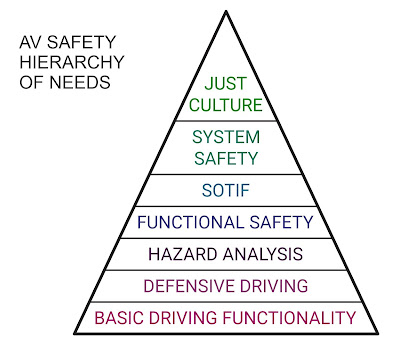
\includegraphics[width=.5\linewidth]{Figures/koopman_pyramid.jpeg}
    \caption{Autonomous Vehicle Safety Hierarchy of Needs from Koopman\cite{koopman}. SOTIF = safety of the intended function.}
    \label{fig:koopman_pyramid}
\end{figure}
